\chapter{Aplikacja do rozpoznawania gestów}
Projekt zakładał utworzenie aplikacji do rozpoznawania gestów w czasie rzeczywistym. Aplikacja została zaimplementowana za pomocą środowiska Visual Studio 2015, w którym utworzono projekt WPF. Jak opisano w podrozdziale \ref{sec: WPF}, WPF to silnik graficzny do tworzenia aplikacji okienkowych, gdzie odpowiednie graficzne elementy oraz widoki są konstruowane za pomocą języka znaczników XAML. Język C\# posłużył do implementacji \textit{back-end'u} aplikacji, wykorzystano również elementy biblioteki Accord .NET, do których należały m.in. funkcje do obsługi kamery oraz filtracji obrazu, algorytm SURF jak również klasyfikator SVM. Dla części widocznej ze strony użytkownika zastosowano zestaw narzędzi o~nazwie \textit{MahApps.Metro}, który nadpisuje domyślny styl graficznych elementów w silniku WPF.

\begin{figure}[h]
	\centering
	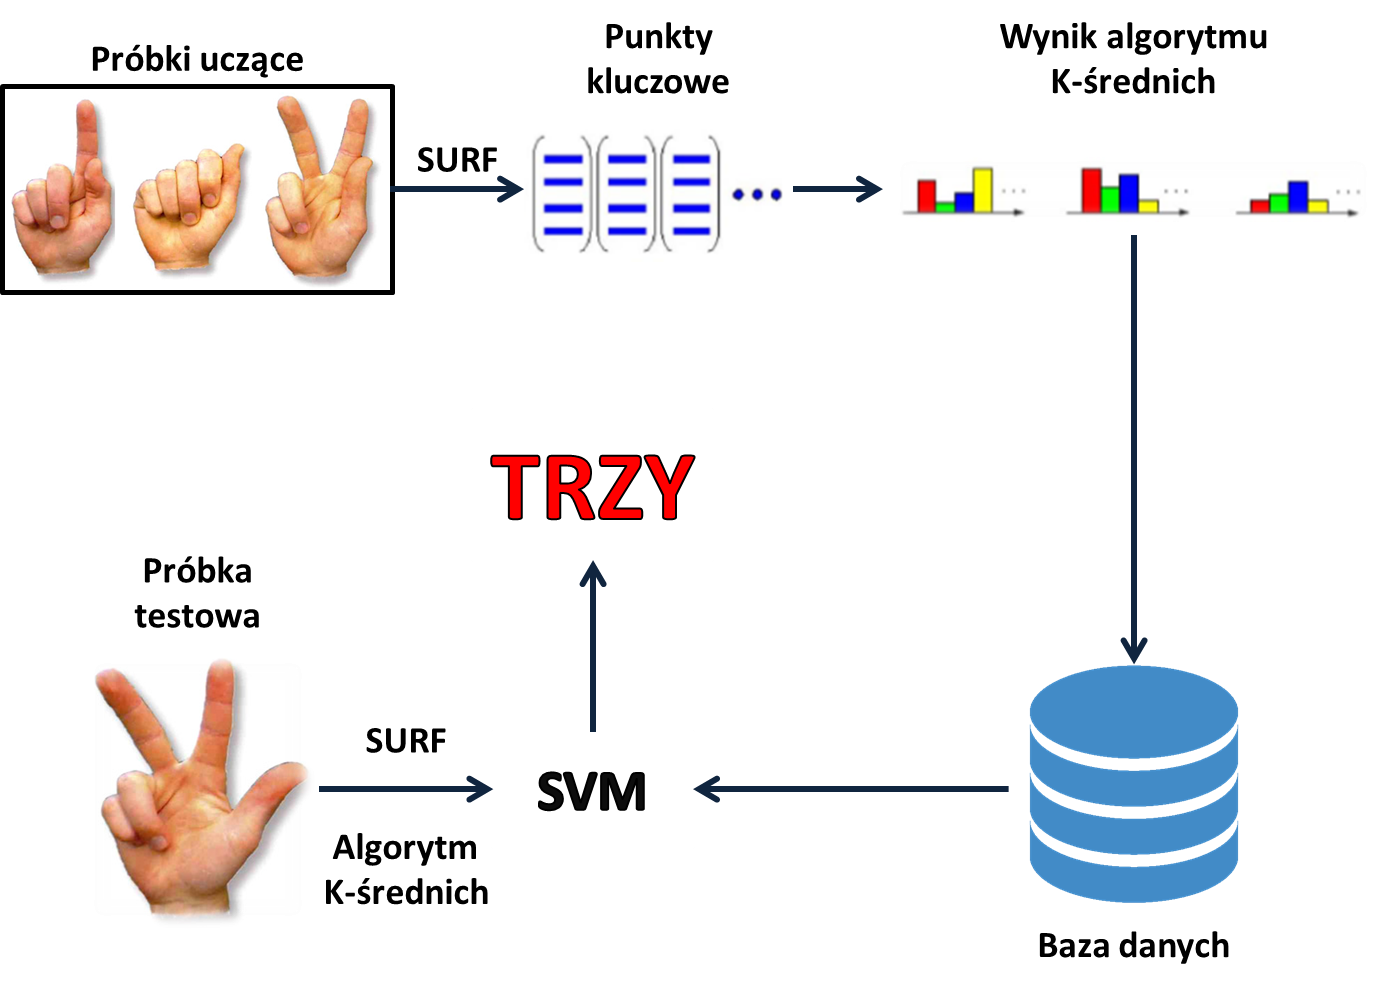
\includegraphics[width=16cm]{ApplicationFlowChart}
	\centering
	\caption{Schemat działania aplikacji.}
	\label{im: ApplicationFlowChart}
\end{figure}

Zasada działania aplikacji została przedstawiona na rysunku \ref{im: ApplicationFlowChart}. Próbki treningowe wraz z odpowiednimi etykietami są poddawane działaniu algorytmu SURF. Wynik operacji to zbiór punktów kluczowych dla każdego z obrazów. Następnie dokonywane jest grupowanie odpowiednich punktów w~znaną z~góry liczbę klastrów. Wyniki grupowania lądują w bazie danych, która jest wykorzystywana do utworzenia modelu SVM. 
Próbka testowa poddawana jest takim samym operacjom co wszystkie próbki uczące - jest ona przekształcana za pomocą algorytmów SURF oraz K-średnich w wektor o znanej liczbie klastrów. Model SVM klasyfikuje próbkę do jednej z podanych kategorii. 

W dalszej części rozdziału przedstawiono szczegółową implementację aplikacji. Pierwszy podrozdział zawiera opis wykorzystanych wzorców projektowych. W kolejnych podrozdziałach opisano każdy z widoków dostępnych w aplikacji wraz ze wzajemnymi zależnościami pomiędzy nimi.

\section{Wzorzec MVVM}
Wzorzec MVVM (skrót od ang. \textit{Model-View-ViewModel}) jest jednym z wzorców architektonicznych służący do tworzenia oprogramowania. Daje możliwość pełnej separacji interfejsu użytkownika od modelu aplikacji. Twórcami wzorca są architekci firmy \textit{Microsoft} Ken Cooper oraz Ted Peters, którzy pracowali nad sposobem usprawnienia programowania sterowanego zdarzeniami. Wzorzec ten stał się jednym z komponentów nowo powstałego silnika graficznego WPF. 
W skład wzorca MVVM wchodzą następujące elementy:
\begin{itemize}
	\item Model: Reprezentuje prawdziwą zawartość aplikacji lub stanowi warstwę dostępu do danych.
	\item View (widok): jest to struktura, którą użytkownik widzi na ekranie swojego monitora.
	\item ViewModel: abstrakcyjna warstwa dla widoku udostępniająca publiczne własności oraz komendy. Za pomocą techniki \textit{data binding} widok wymienia informację z powiązanym z nim ViewModelem. ViewModel odpytuje model w celu pobrania lub zmiany danych. Zastosowanie struktury ViewModelu eliminuje istnienie bezpośredniego połączenia pomiędzy widokiem a modelem.
\end{itemize}

\section{Wzorzec Mediator}
\label{sec: mediator}
W inżynierii oprogramowania mediator jest wzorcem projektowym należącym do grupy wzorców czynnościowych. Jest jednym z 23 wzorców projektowych opisanych przez tzw. \textit{"Bandę Czworga"} (z~ang. \textit{Gang of Four}, GoF) w książce \textit{"Design Patterns: Elements of Reusable Object-Oriented Software"} stanowiącej jeden z kanonów tworzenia oprogramowania. Zastosowanie wzorca powoduje, że komunikacja pomiędzy obiektami jest zawarta w obiekcie mediatora. Obiekty nie komunikują się bezpośrednio ze sobą, lecz wykorzystują mediatora do pośredniej komunikacji, który koordynuje wzajemną interakcję.  Dzięki temu następuje redukcja wzajemnych zależności pomiędzy komunikującymi się obiektami. Klasa klienta może wykorzystać mediatora w celu wysłania wiadomości do innych klientów oraz może otrzymać powiadomienie zwrotne poprzez zdarzenie pochodzące od klasy mediatora. Obiekty są w ten sposób luźno powiązane pomiędzy sobą, dzięki temu komunikacja jest łatwa w implementacji. Testowanie oraz ponowne wykorzystanie kodu jest możliwe, ponieważ obiekty muszą jedynie odnosić się do mediatora oraz nie posiadają żadnej informacji o innych elementach.

\section{Architektura aplikacji}
Architektura aplikacji została przedstawiona na rysunku \ref{im: AppArchitectureWithHsl}. Składa się ona z trzech klas stanowiących model, czterech widoków oraz z powiązanymi z nimi modelami widoków. 

\begin{figure}[h!]
	\centering
	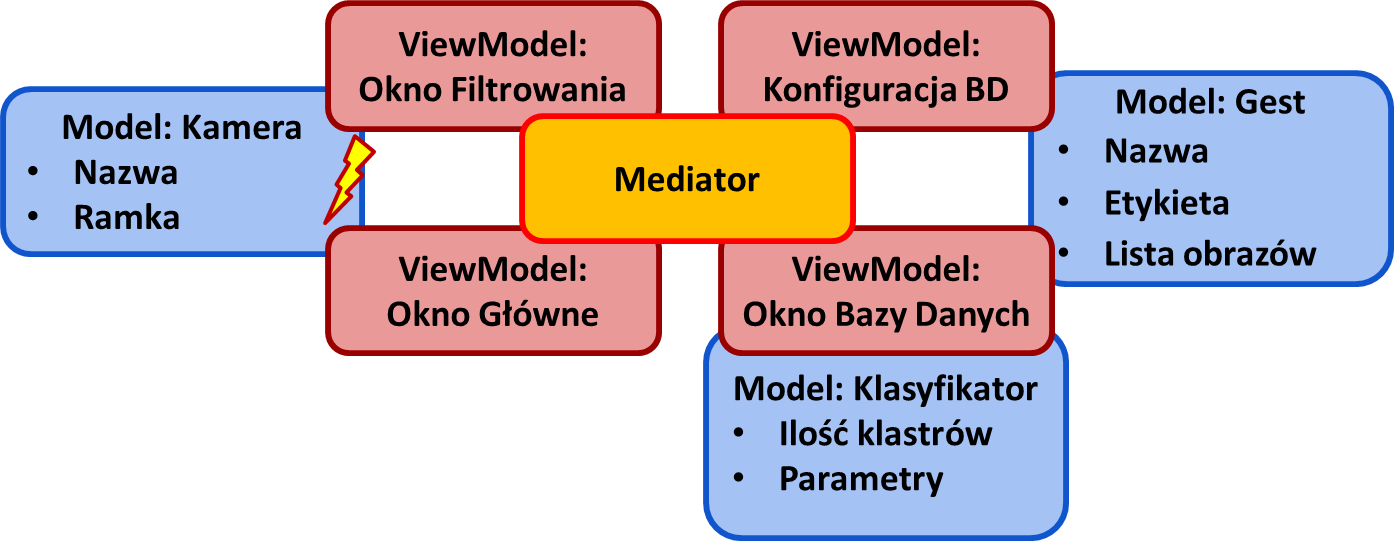
\includegraphics[width=16cm]{ArchitectureMediator}
	\centering
	\caption{Architektura aplikacji.}
	\label{im: AppArchitectureWithHsl}
\end{figure}

W skład modelu wchodzi klasa \textit{Camera} posiadająca flagę informującą o stanie urządzenia (czy jest włączone) oraz właściwości opisujące nazwę kamery oraz bieżącą ramkę. Model ten jest powiązany z~dwoma modelami widoków: z oknem głównym oraz z oknem służącym do filtrowania obrazu w przestrzeni barw HSL. Model kamery informuje widoki modelu o zmianie swoich właściwości za pomocą zdarzenia. Zmiana kamery lub jej właściwości jest możliwa jedynie za pomocą głównego okna aplikacji. Kolejną częścią modelu jest klasa powiązana z gestem. Posiada właściwości opisujące nazwę gestu, etykietę oraz zawiera listę wektorów opisujących każdy obraz wchodzący w skład gestu. Model ten jest powiązany z widokiem modelu dla bazy danych, jak również z pomocniczym widokiem służącym do konfiguracji bazy danych. Ostatni element modelu to klasa powiązana z klasyfikatorem. Posiada własności odpowiedzialne za liczbę klastrów czy parametry modelu SVM. Zmiana parametrów tej klasy jest możliwa wyłącznie za pomocą widoku modelu skojarzonym z bazą danych.

Wymiana informacji pomiędzy modelami widoków zachodzi z wykorzystaniem opisanego w sekcji \ref{sec: mediator} mediatora. Dzięki niemu elementy aplikacji są ze sobą luźno powiązane i ewentualna zmiana w~architekturze aplikacji jest łatwo wykonywalna. 

\begin{figure}[h!]
	\centering
	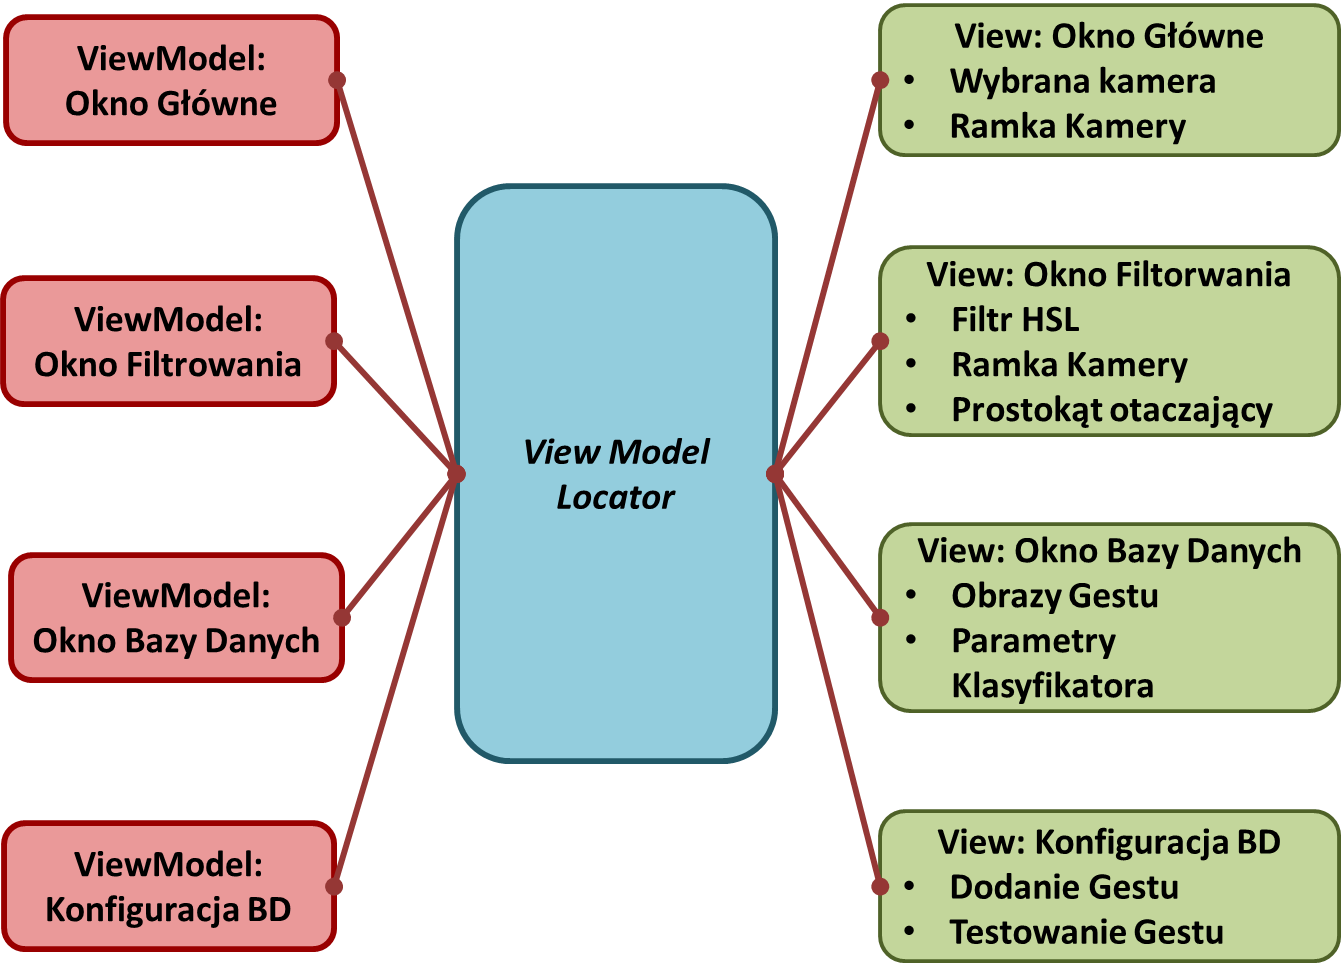
\includegraphics[width=14cm]{ViewModelLocator}
	\centering
	\caption{\textit{View Model Locator}.}
	\label{im: ViewModelLocator}
\end{figure}

Powiązanie pomiędzy modelem widoku a widokiem wykorzystuje wzorzec projektowy o nazwie \textit{View Model Locator} (rysunek \ref{im: ViewModelLocator}). Wykorzystanie tego wzorca stanowi standardowy, spójny oraz deklaratywny sposób powiązania widoku z modelem widoku  w podejściu \textit{view first}. Zasada łączenia widoku modelu z widokiem można opisać następującymi krokami:
\begin{enumerate}
	\item \textit{View Model Locator} sprawdza jaki widok ma zostać stworzony.
	\item Wzorzec identyfikuje widok modelu dla  tworzonego widoku.
	\item \textit{View Model Locator} konstruuje widok modelu.
	\item Wysłanie danych ustawionych w widoku do \textit{View Model'u}.
\end{enumerate}

Baza danych jest w postaci pliku XML (skrót on ang. \textit{Extensible Markup Language}). Zawiera ona informacje o wszystkich gestach dostępnych w bazie. Każdy węzeł występujący w pliku posiada dwa atrybuty: nazwę gestu oraz numer etykiety. Wewnątrz każdego węzła znajdują się rekordy, które są mapowane na  poszczególne obrazy w obrębie gestu. Pojedynczy rekord posiada dwa atrybuty: nazwę pliku oraz wektor cech opisujący dany gest.

\subsection{Główny widok aplikacji}
Na rysunku \ref{im: MainWindow} przedstawiono widok główny aplikacji do rozpoznawania gestów. W jego skład wchodzą następujące elementy:
\begin{itemize}
	\item Bieżąca ramka kamery. Jest to element stanowiący największą część głównego okna. Odświeżanie obrazu zachodzi po każdym zdarzeniu wynikającym z pojawienia się nowej ramki w modelu kamery.
	\item Lista rozwijana, której elementy reprezentują urządzenia wideo podłączone do komputera. Zmiana kamery możliwa jedynie w przypadku, gdy obecnie wybrana kamera jest rozłączona.
	\item Element umożliwiający zmianę rozdzielczości dla wybranej kamery. Zmiana jest możliwa jedynie w przypadku, gdy wybrana kamera nie rejestruje strumienia wideo.
	\item Przyciski \textit{CONNECT} oraz \textit{DISCONNECT}. Odpowiadają za start oraz zatrzymanie wybranej kamery. W przypadku, gdy kamera jest uruchomiona, niemożliwe jest użycie przycisku związanego ze startem kamery. Analogiczne zachowanie występuje dla przycisku \textit{DISCONNECT}.
	\item Przycisk \textit{TAKE SNAPSHOT}. Naciśnięcie przycisku powoduje pobranie prostokąta otaczającego stanowiącego część bieżącej ramki ze strumienia wideo. Prostokąt zostaje wysłany do widoku modelu powiązanego z bazą danych, gdzie zachodzi jego klasyfikacja oraz przypisanie do istniejącego gestu. Działanie jest możliwe wyłącznie wtedy, gdy wybrana kamera jest włączona oraz gdy w bazie danych jest więcej niż jeden gest. 
	\item Przycisk \textit{SET HSL FILTER}. Otwarcie okna, w którym możliwa jest edycja składowych filtra przestrzeni barw HSL. Szczegóły w podrozdziale \ref{subsec: HslFIlter}.
	\item Przycisk \textit{OPEN DATABASE}. Naciśnięcie przycisku otwiera widok bazy gestów. Szczegółowe informacje o zachowaniu widoku bazy są dostępne w podrozdziale \ref{subsec: Database}.
\end{itemize}

\begin{figure}[h!]
	\centering
	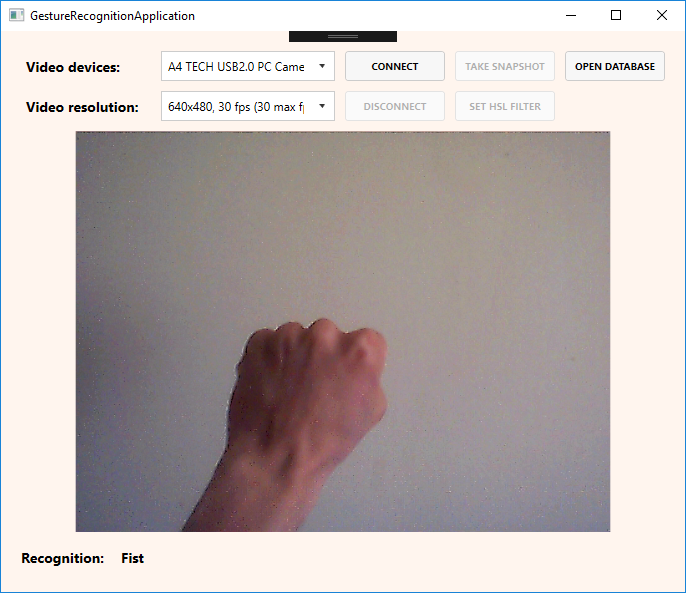
\includegraphics[width=12cm]{MainWindow}
	\centering
	\caption{Widok główny aplikacji}
	\label{im: MainWindow}
\end{figure}

\subsection{Okno filtrowania}
\label{subsec: HslFIlter}
Okno filtrowania zostało przedstawione na rysunku \ref{im: HslWindow}. Podobnie jak w  przypadku głównego okna, najważniejszy element stanowi obraz z bieżącą ramką kamery. Powyżej ramki znajdują się elementy związane z filtrowaniem przestrzeni barw HSL. Istnieje możliwość zmian zakresu wartości poszczególnej składowej, a wyniki tych operacji są widoczne na ramce kamery. Wyliczanie obrazu z nałożonym filtrem następuje po każdym zdarzeniu powiązanym z pojawieniem się nowej ramki w modelu kamery.
Obraz jest tworzony w taki sposób, że jeżeli dany piksel z oryginalnego obrazu spełnia kryteria nałożonego filtru, to taki piksel zostaje wyświetlony. W przeciwnym wypadku przypisuje mu się wartość koloru czarnego. Dodatkowo na obszarze obrazu zastosowano prostokąt otaczający, który obejmuje największy element znaleziony po etapie filtrowania. Następnie prostokąt zostaje wysłany do widoku głównego i~tam wyświetlony na obrazie oryginalnym.
\begin{figure}[h!]
	\centering
	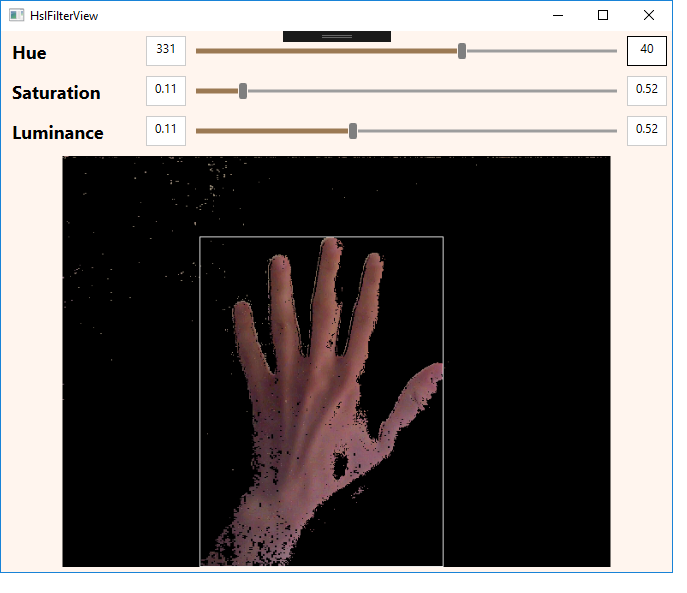
\includegraphics[width=14cm]{HslWindow}
	\centering
	\caption{Okno filtrowania przestrzeni HSL.}
	\label{im: HslWindow}
\end{figure}
 
\newpage 
\subsection{Okno bazy danych}
\label{subsec: Database}
Na rysunku \ref{im: DatabaseWidow} przedstawiono okno bazy danych dla aplikacji rozpoznawania gestów. W obrębie okna można wyodrębnić dwa główne elementy: widok zakładek oraz panel umożliwiający konfigurację bazy danych. 

\begin{figure}[h!]
	\centering
	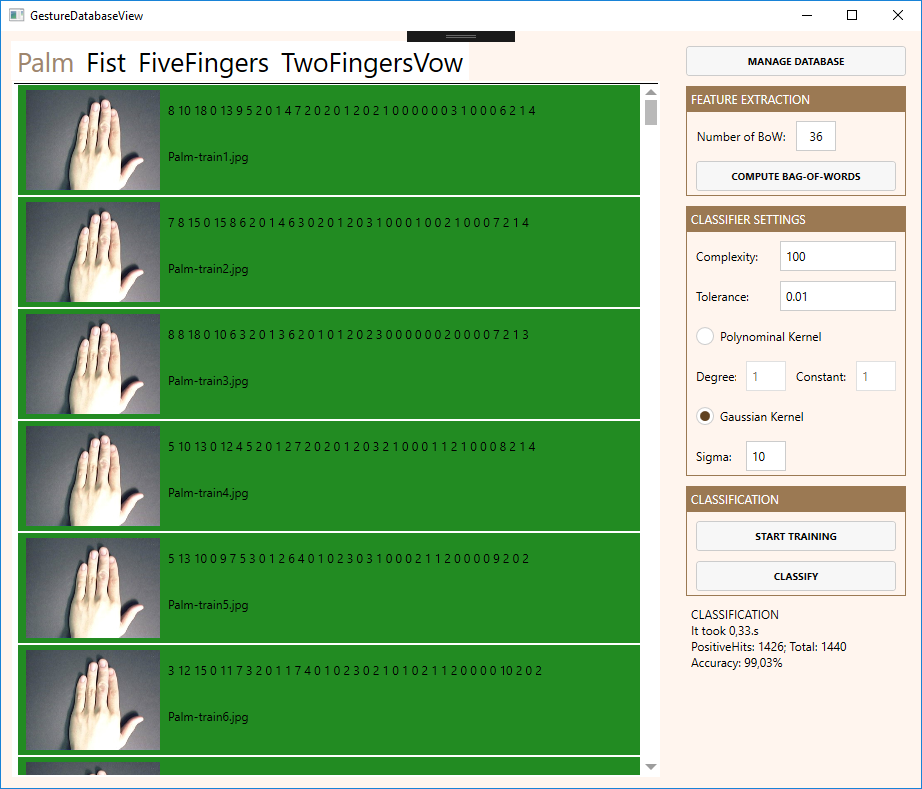
\includegraphics[width=16cm]{DatabaseWidow}
	\centering
	\caption{Okno bazy gestów.}
	\label{im: DatabaseWidow}
\end{figure}

Wszystkie gesty dostępne w bazie są widoczne w widoku zakładek. Nazwy gestów stanowią nagłówki, które użytkownik może przełączać w celu zaciągnięcia informacji o danym geście. Pojedyncza zakładka zawiera listę elementów, a każdy rekord składa się ze zdjęcia gestu, nazwy pliku oraz deskryptora opisującego pojedynczy gest. Dodatkowo kolor tła dla każdego elementu informuje,czy dany obraz został poprawnie sklasyfikowany.

Po prawej stronie okna umieszczono panel służący do konfiguracji bazy gestów. Pierwszy element stanowi przycisk umożliwiający konfigurację bazy danych. Po jego kliknięciu zostaje otworzony widok, w którym użytkownik może wczytać pliki zawierające gesty jak również dokonać ich klasyfikacji. W przypadku, gdy nazwa wczytywanego gestu istnieje w bazie, obrazy zostaną dodane właśnie do tego elementu bazy danych. 

Pierwsza grupa elementów umieszczona poniżej przycisku do zarządzania bazą danych powiązana jest z ekstrakcją cech. W jej skład wchodzi edytowalne pole numeryczne, w którym użytkownik podaje długość wektora cech. Drugi element to przycisk służący do wyliczania deskryptora. Po jego kliknięciu wszystkie obrazy z bazy danych są poddawane działaniu algorytmu SURF, który wylicza ekstrema dla każdego z nich. Aby wszystkie obrazy były opisane przez deskryptor o takiej samej długości, konieczne jest zastosowanie algorytmu k-średnich. Algorytm ten tworzy klastry, których liczba jest wprowadzana przez użytkownika.

Kolejna grupa właściwości jest powiązana z ustawieniami klasyfikatora. W aplikacji wykorzystano dostępny w bibliotece Accord.NET klasyfikator rozwiązujący problem klasyfikacji dla wielu kategorii. Użytkownik ma możliwość wyboru pomiędzy metodami tzw. \textit{kernel tricku'u} opisanego w podrozdziale \ref{sec: SVM}. W aplikacji zaimplementowano wielomianową niejednorodną funkcję jądra oraz metodę opartą o jądro RBF. Dla metody wielomianowej użytkownik ma możliwość podania stopnia wielomianu oraz stałej, a dla metody opartej o rozkład Gaussa jest możliwa zmiana parametru $\sigma$. Dla obu metod istnieje możliwość konfiguracji dwóch parametrów: parametru dla funkcji kary, która zostaje nałożona w przypadku złej klasyfikacji próbek treningowych oraz tolerancji, której wartość stanowi kryterium stopu podczas uczenia klasyfikatora SVM. 

\begin{figure}[h!]
	\centering
	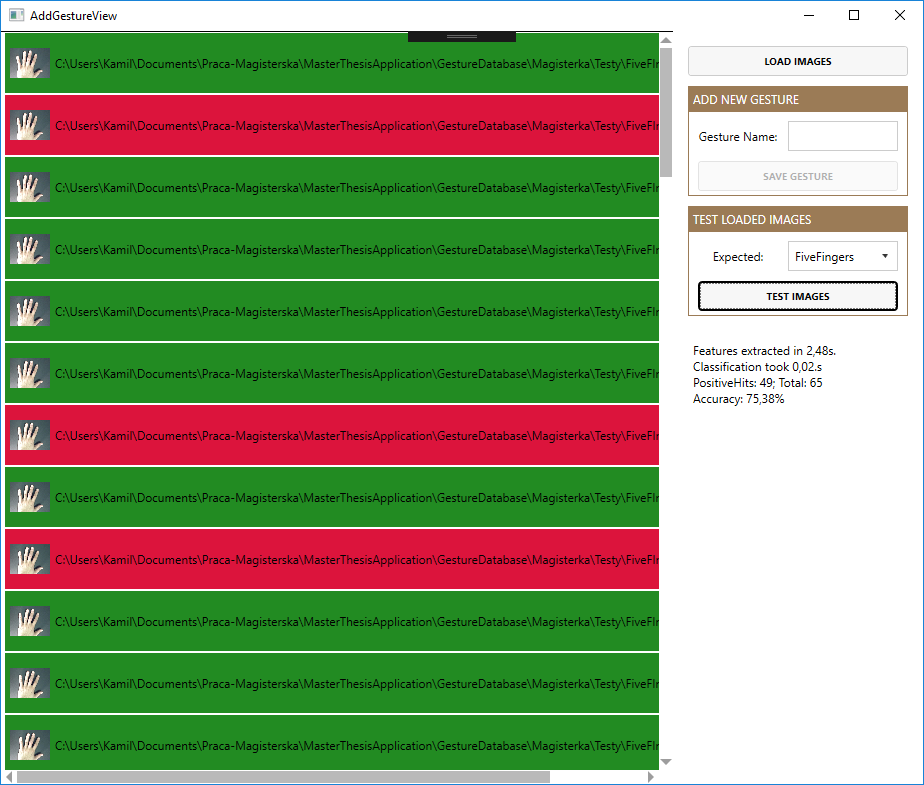
\includegraphics[width=16cm]{ManageDatabaseWindow}
	\centering
	\caption{Okno konfiguracji bazy danych wraz z możliwością testowania obrazów.}
	\label{im: ManageDatabaseWindow}
\end{figure}

Kolejne dwa przyciski są powiązane z uczeniem modelu SVM oraz do klasyfikacji próbek treningowych.  Dla każdego obrazu gestu z widoku zakładek po procesie klasyfikacji zostaje przypisany kolor tła: zielony w przypadku poprawnego rezultatu, czerwony dla złego. Dodatkowo, gdy oba procesy zostaną wykonane, na ekranie wyświetlane są informacje dotyczące czasu trwania klasyfikacji oraz jej dokładności. Są one wykorzystane podczas porównywania działania klasyfikatora dla różnych wartości parametrów.

Jak wspomniano powyżej, przycisk \textit{MANAGE DATABASE} służy do zarządzania bazą danych. Po jego kliknięciu ukazuje się widok przedstawiony na rysunku \ref{im: ManageDatabaseWindow}. W celu dodania gestów do bazy danych, użytkownik musi wczytać przynajmniej jeden obraz oraz podać jego nazwę. W przypadku, gdy nazwa istnieje w bazie danych, obrazy zostaną automatycznie dodane na koniec listy związanej z danym gestem.
Dodatkowo istniej możliwość klasyfikacji wczytanych obrazów. W tym celu użytkownik może wybrać istniejący gest z bazy danych i sprawdzić, z jaką skutecznością wczytane obrazy są klasyfikowane. Podobnie jak dla widoku bazy danych, kolor tła oznacza wynik klasyfikacji: zielony w przypadku, gdy klasyfikacja przebiegła pomyślnie, czerwony dla błędnego przypisania. Poniżej przycisków widnieje okno wyświetlające informacje o czasie działania algorytmu oraz o jego dokładności.




























